\documentclass[bare_jrnl_transmag]{subfiles}
\begin{document}

\subsection{System Architecture}

The overall architecture for the algorithm can be broken into two parallel steps. On one side, the IMU data is read, and the pose is estimated using the Madgwick filter. The estimated pose and new acceleration from the IMU are fed into the Kalman Filter as the new states to determine a predicted new position. 

On the other side, the camera data is processed and filtered for features to determine changes in position, which are fed into the Kalman filter as the measurements.

The Kalman filter fuses the two sensor inputs together to generate the new pose and position of the drone. 

Figure \ref{fig:vio-arch} shows the overall architecture of the algorithm. 

\begin{figure}
    [H]
    \centering
    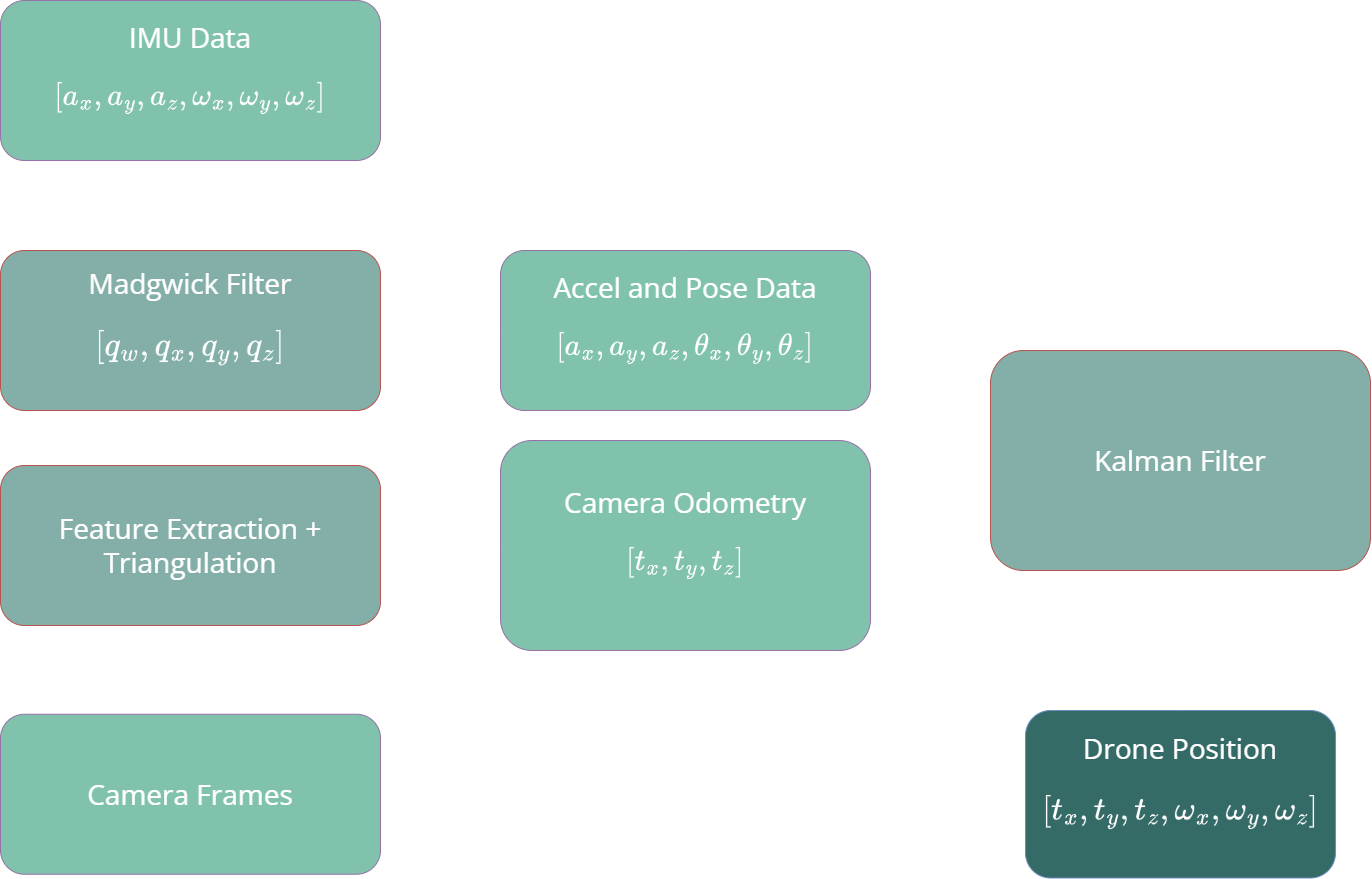
\includegraphics[width=0.8\linewidth]{figures/VIO-arch.png}
    \caption{VIO Algorithm architecture}
    \label{fig:vio-arch}
\end{figure}


\end{document}